%Presentation on numerical differentiation 

\documentclass{beamer}

\mode<presentation>
{
  \usetheme{default}      
  \usecolortheme{default} 
  \usefonttheme{default}  
  \setbeamertemplate{navigation symbols}{}
  \setbeamertemplate{caption}[numbered]
} 

\usepackage[english]{babel}
\usepackage[utf8x]{inputenc}
\usepackage{graphicx}
\usepackage{listings}
\usepackage{color}

\title[Numerical Differentiation]{Numerical Differentiation}
\author{Omer F Koru and Ethan Feilich}
\institute{University of Pennsylvania}
\date{\today}

\definecolor{mygreen}{rgb}{0,0.6,0}
\lstset{language=Matlab,%
	%basicstyle=\color{red},
	breaklines=true,%
	commentstyle=\color{mygreen}, 
	keywordstyle=\color{blue},%
	numbers=left,%
	numberstyle={\tiny \color{black}},% size of the numbers
	numbersep=9pt, % this defines how far the numbers are from the text
	emph=[1]{for,end,break},emphstyle=[1]\color{red}, %some words to emphasise
	frame=single,
}

%Beginning of presentation

\begin{document}

\begin{frame}
  \titlepage
\end{frame}

\begin{frame}
\frametitle{Basic Concepts}

Why numerical differentiation?\\
\hfill\\

\begin{itemize}
\setlength\itemsep{1em}
\item We have a function we'd like to differentiate, but we only have function values at discrete points
\item We'd like to study changes in data, where it may not be obvious that an underlying function exists
\item Exact formulas for a function may be available, but computationally expensive
\item Discrete approximating solutions to differential equations are defined on a grid, and we need to evaluate derivatives at the grid points
\end{itemize}

\end{frame}

\begin{frame}
\frametitle{Centered Differencing}

\begin{align*}
f'(x) &\approx \frac{f(x+h) - f(x)}{h} & & \textrm{``forward differencing''}\\
\uncover<2->{f'(x) &\approx \frac{f(x) - f(x-h)}{h} & & \textrm{``backward differencing''}}\\
\uncover<3->{f'(x) &\approx \frac{f(x+h) - f(x-h)}{2h}& & \textrm{``centered differencing''}}
\end{align*}

\hfill\\

\uncover<4->{Centered differencing carries a smaller truncation error which converges ``faster''.}

%Centered differencing produces approximation error of order O(h^2) as opposed to other methods where approximation error is of order O(h).

\end{frame}

\begin{frame}
	\frametitle{Error for Different h}
	\begin{figure}
		\centering
			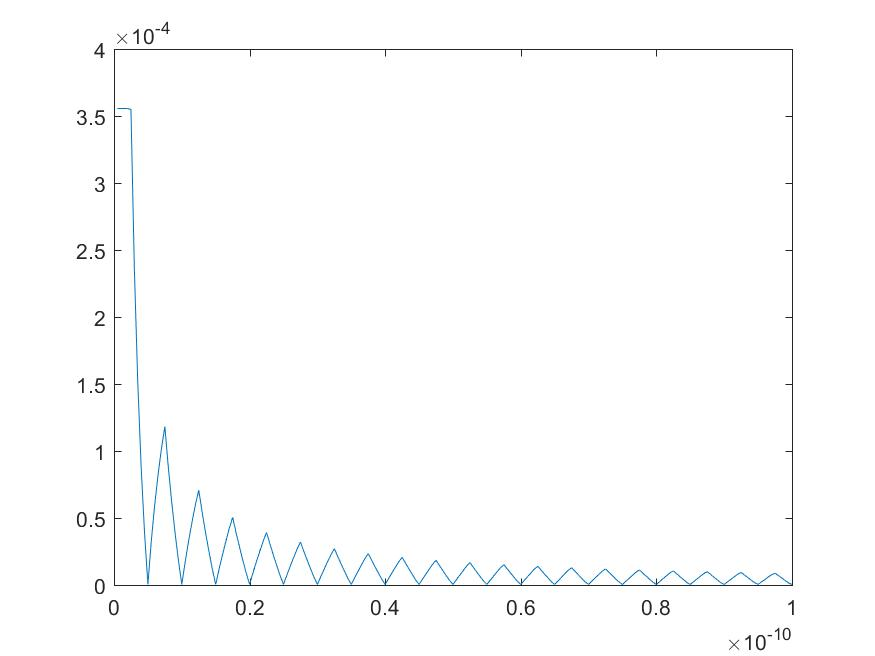
\includegraphics[scale=0.3]{error_diff_sqrt_x}
	\end{figure}
	$f(x) = x^2$, derivative at $2$ with forward differencing\\
	$h$ from $10^{-12}$ to $10^{-10}$
%	Smaller $h$ higher error!
\end{frame}


\begin{frame}
\frametitle{Optimal Choice of h}

To minimize the sum of round-off and truncation error, choose $h=h^*$ by

\begin{align*}
h = \sqrt{\frac{\epsilon_f f}{f''}} \approx \sqrt{\epsilon_f}x_c
\end{align*}
\hfill\\
\hfill\\
where $\epsilon_f$ is the fractional accuracy with which $f$ is computed.  Without information about $f$ and $f''$ we typically assume $x_c = x$.

\end{frame}

\begin{frame}
\frametitle{Interpolation}

Assuming we have $f(x_0),\ldots, f(x_n)$, the Lagrange form of the interpolation polynomial is:

\begin{align*}
Q_n(x) = \sum_{j=0}^n f(x_j) l_j(x)
\end{align*}

The numerical differentiation formula, derived from the interpolation error formula is:
%Discuss derivation of this formula from differentiation of interpolation error formula.  

\begin{align*}
f'\left( x_{k}\right) &=\sum _{j=0}^{n}f\left( x_{j}\right) l'_{j}\left( x_{k}\right)+\dfrac {1} {\left( n+1\right) !}f^{\left( n+1\right) }\left( \xi _{x_{k}}\right)  \prod _{\substack{j=0\\j\neq k}}\left( x_{k}-x_{j}\right) \\
%&= Q'_n(x_k) + \dfrac {1} {\left( n+1\right) !}f^{\left( n+1\right) }\left( \xi _{x_{k}}\right)  \prod _{\substack{j=0\\j\neq k}}\left( x_{k}-x_{j}\right)
\end{align*}

where $\xi_{x_k}\in  (min(x, x_0, . . . , x_k), max(x, x_0, . . . , x_k)). $
\end{frame}

\begin{frame}
\frametitle{Undetermined Coefficients}

The method of undetermined coefficients is described by the algorithm:\\
\hfill\\

\begin{itemize}
\setlength\itemsep{1em}
\item Express the derivative as a linear combination of function values at certain points
\item Derive the Taylor expansions of the function at the approximation points
\item Equate the coefficients of the function and its derivatives on both sides
\end{itemize}

\end{frame}

\begin{frame}
\frametitle{Undetermined Coefficients}

Suppose we have three points, then the linear combination and Taylor approximation around $x_1$ are:

\begin{align*}
f'(x_1) &\approx af(x_1) + bf(x_2) + cf(x_3)\\
f(x_i) &= f(x_1) + f'(x_1)(x_i - x_1) + \frac{f''(x_1)(x_i-x_1)^2}{2}+\frac{(x_i-x_1)^3 f'''(\xi_i)}{6}
\end{align*}
\hfill\\
\hfill\\
for $i = 2,3$ and $\xi_i \in (x_1,x_i)$.  Solving for a,b, and c gives the 3x3 system:

\begin{align*}
a+b+c=0\\
b(x_2-x_1) + c(x_3-x_1) = 1\\
b(x_2-x_1)^2 + c(x_3-x_1)^2 = 0
\end{align*}

\end{frame}

\begin{frame}
\frametitle{Richardson’s Extrapolation}

%Richardson's extrapolation is a method used to improve approximation accuracy by incorporating additional points, assuming the structure of the error is known.\\
%\hfill\\
Let $L = f'(x)$. The truncation error from the center differencing approximation has the form:

\begin{align*}
L &= \frac{f(x+h) - f(x-h)}{2h} - \left[ \frac{h^2}{3!}f^{(3)}(x) + \frac{h^4}{5!}f^{(5)}(x) \right] + \ldots \\
&= D(h) + e_2h^2 + e_4 h^4 + \ldots
\end{align*}
\hfill\\ \hfill\\
where the coefficients $e_k$ don't depend on $h$.  

\end{frame}

%\sum_{k=0}^\infty \frac{f^{(k)}(x)}{k!}h^k - \sum_{k=0}^\infty \frac{(-1)^k f^{(k)}(x)}{k!}h^k

\begin{frame}
\frametitle{Richardson’s Extrapolation}

The approximation can be improved by incorporating more points.

\begin{align*}
L &= D(2h) + e_2(2h)^4 + e_4(2h)^4 + \ldots\\
4L &= 4D(2h) + 4e_2(2h)^4 + 4e_4(2h)^4 + \ldots\\
\end{align*}

Subtracting the two approximations gives:

\begin{align*}
L = \frac{4D(h) - D(2h)}{3} - 4e_4h^4 + \ldots
\end{align*}

Which eliminates the $e_2h^2$ term from the error.  The resulting fourth order approximation is:

\begin{align*}
f'(x) = \frac{−f(x + 2h) + 8f(x + h) − 8f(x − h) + f(x − 2h)}{12h} + O(h^4)
\end{align*}

\end{frame}



\begin{frame}[fragile]
	\frametitle{Symbolic Differentiation}
	\begin{lstlisting}[tabsize=8,basicstyle=\footnotesize]
	%symbolic variables
	syms a
	% symbolic function
	g=  log(a+5)*a^2*exp(sqrt(a));
	% symbolic diff
	dg = diff(g);
	display(dg);
	% evaluation of diff at x=2
	a=2;
	%substitute a=2 to dg
	eval(subs(dg))
	\end{lstlisting}

	\begin{equation*}
		g(a) = log(a+5) \times a^2 \times e^{\sqrt{a}}
	\end{equation*}

	\begin{verbatim}
	dg =
	2*a*log(a + 5)*exp(a^(1/2))+(a^2*exp(a^(1/2)))/(a + 5)+
	(a^(3/2)*log(a+5)*exp(a^(1/2)))/2
	\end{verbatim}
%	
\end{frame}

\end{document}
